\documentclass[tikz,border=6pt]{standalone}
\usetikzlibrary{patterns,arrows.meta,calc}
\begin{document}
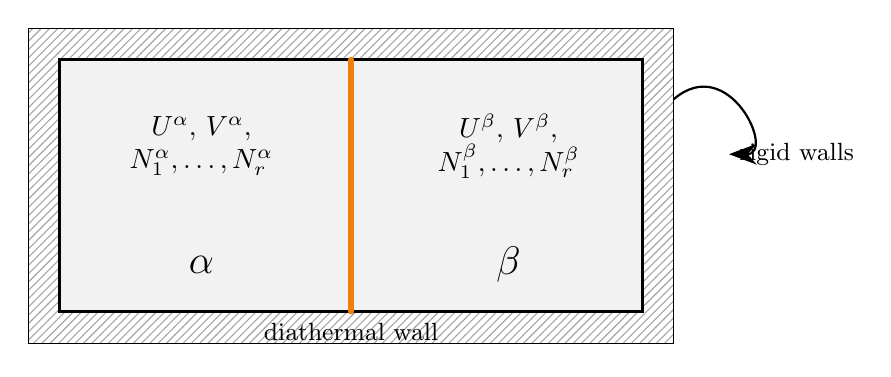
\begin{tikzpicture}[line cap=round]
  % Styles and colors
  \tikzset{
    rigid/.style={pattern=north east lines, pattern color=gray!70},
    wall/.style={line width=1.2pt},
    diathermal/.style={line width=2pt,draw=orange!75!brown},
    label/.style={font=\small}
  }
  \colorlet{wallfill}{gray!10}

  % Outer rigid shell
  \draw[rigid] (0,0) rectangle (8.2,4);
  % Inner cavity
  \fill[wallfill] (0.4,0.4) rectangle (7.8,3.6);
  \draw[wall] (0.4,0.4) rectangle (7.8,3.6);

  % Diathermal wall
  \draw[diathermal] (4.1,0.4) -- (4.1,3.6);

  % Left subsystem (alpha)
  \node[align=center] at (2.2,2.5) {$U^\alpha,\,V^\alpha,$ \\ $N_1^\alpha,\ldots,N_r^\alpha$};
  \node[font=\Large] at (2.2,1.0) {$\alpha$};

  % Right subsystem (beta)
  \node[align=center] at (6.1,2.5) {$U^\beta,\,V^\beta,$ \\ $N_1^\beta,\ldots,N_r^\beta$};
  \node[font=\Large] at (6.1,1.0) {$\beta$};

  % Labels
  \node[align=center,font=\small] at (4.1,0.15) {diathermal wall};

  \draw[-{Stealth[length=10pt]},thick]
    ($(8.2,3.1)$) .. controls +(0.7,0.6) and +(0.6,0.0) .. ($(8.9,2.4)$)
    node[right,label] {rigid walls};
\end{tikzpicture}
\end{document}
